\chapter{Introducción}
\label{cap:introduccion}

\chapterquote{Todo se hunde en la niebla del olvido pero cuando la niebla se despeja, el olvido está lleno de memoria}{Mario Benedetti}

\section{Motivación}

Nuestra existencia se compone esencialmente de vivencias, momentos únicos y personales que marcan el recorrido en la vida de cada uno. Nuestra identidad se forma con el conjunto de los eventos que vamos experimentando en el camino y para preservarlos, el cerebro los va almacenando en forma de recuerdos a lo largo de toda nuestra vida.  Desde nuestro primer recuerdo, que normalmente está comprendido entre los 2 y 4 años, debido a que la formación de nuevas neuronas impide que el hipocampo almacene recuerdos hasta esa edad, fenómeno que se conoce como amnesia infantil (Freud, 1895). Hasta el último, el cual puede darse el caso de ser distorsionado o borrado completamente debido al deterioro de nuestro cerebro y la imposibilidad de nuestras neuronas a realizar las conexiones posibles para ello. Este último caso incluye a una enfermedad degenerativa comúnmente conocida como Alzheimer, que actualmente afecta a más de 55 millones de personas en todo el mundo. Sin embargo, no son sólo estas personas quiénes la sufren, sino todos sus allegados también. \\

\section{¿Qué es el Alzheimer?}

El Alzheimer es una enfermedad que destruye lentamente la memoria y que, además, también va deteriorando los pensamientos y la conducta, hasta que poco a poco se ven afectadas las funciones más básicas. El Alzheimer es la principal causa de la demencia \citep{NationalInstitute2023}.\\

El cerebro envía estímulos químicos a través de las neuronas creando conexiones cerebrales, y mediante miles de millones de estas conexiones, se obtienen nuestros recuerdos, sentimientos, pensamientos y capacidades locomotoras. Aunque todavía no se sabe con certeza el motivo que causa esta enfermedad en el cerebro, se ha investigado que hay dos proteínas en el cerebro que con el tiempo se vuelven tóxicas, tau y beta-amiloide, que se acumulan hasta obstruir la conexión entre las neuronas y provocar que estas mueran, como se puede ver en \ref{fig:tau}.  Con la destrucción de las neuronas, el cerebro se va encogiendo y con él también severamente, el hipocampo, que es una parte clave fundamental en nuestro cerebro a la hora de formar nuevos recuerdos y para el aprendizaje, lo que causa que nuestra memoria, nuestra capacidad para tomar decisiones y el habla, fallen. Para ayudar a combatir esta enfermedad existen métodos farmacológicos y no farmacológicos. En este proyecto nos centraremos en el segundo grupo, más concretamente, en la terapia de reminiscencia. \\

\begin{figure}[h]
	\centering
	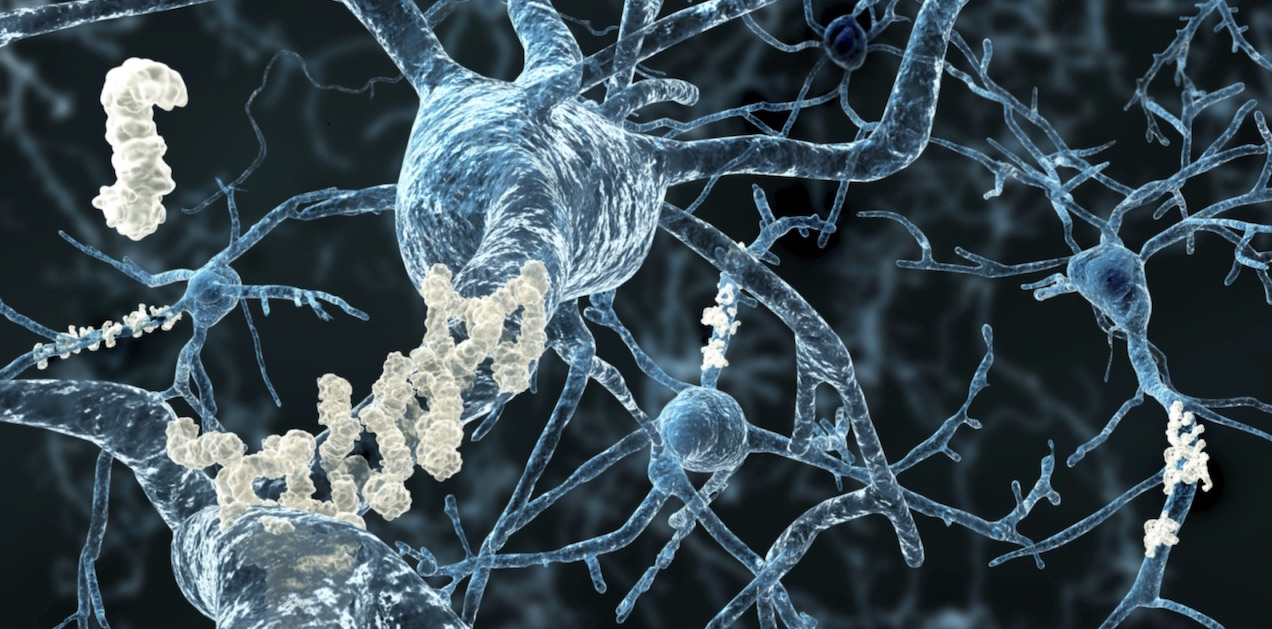
\includegraphics[width = 1 \textwidth]{Imagenes/Vectorial/proteina-tau.jpg}
	\caption{Obstrucción de neuronas por la vitamina tau \citep{tau}}
	\label{fig:tau}
\end{figure}


\section{La terapia de reminiscencia}

Afortunadamente, existen terapias que ayudan a mejorar la calidad de vida de las personas que padecen esta enfermedad. Entre ellas la estimulación cognitiva, orientación a la realidad, ejercicio terapéutico, musicoterapia, y estimulación multisensorial, entre otras \citep{SAS2020}.\\

Nuestro proyecto está ligado a la terapia de reminiscencia, que es un proceso que ayuda a la persona a evocar momentos y experiencias emocionales e integrarlos en el presente, lo cual puede mejorar la autoestima y la calidad de vida \citep{gonzalez2015terapia}.\\

En concreto, la técnica consiste en mostrar a la persona una herramienta o material visual, musical o incluso, olfativo, vinculado a su propia experiencia o hechos históricos. De esta manera se promoverá una revisión de la vida de la persona, de modo que se consiga una conexión con sus vivencias, con el fin de reconstruir un libro de vida y reforzar su identidad como persona.  Esta terapia se puede clasificar como un tipo de ensoñación que los lleva a su pasado, lo que les permite entrar en un estado de concentración con el fin de poder reforzar su memoria general, lo cual fortalece al cerebro y desarrolla sus capacidades sociales, estimula recuerdos a través de órganos sensoriales y activa su sentido de la identidad.\\



Algunos de los beneficios de la creación del libro de vida y la terapia ocupacional de reminiscencia, entre muchos otros, son:\\
\begin{itemize}
	\item \underline{Bienestar emocional}: Se permite que las personas puedan recordar experiencias positivas y significativas de sus vidas, lo cual puede generar sensaciones satisfactorias, de alegría y felicidad.\\
	\item \underline{Autoconocimiento}: Cuando una persona revisa y reflexiona sobre eventos pasados y logros personales, puede obtener una comprensión de sí misma. Mediante la interacción de sus recuerdos, ayudado de la guía de cuidadores y terapeutas, puede evocar aspectos de sus valores, fortalezas y debilidades que de otra manera no serían accesibles.
	\item \underline{Sentido y propósito personal}: Mediante la rememoración de escenas significativas, las personas pueden encontrar una guía emocional que permite dar sentido y dirección a sus vidas, especialmente en momentos de confusión o desorientación.
	\item \underline{Reducción del estrés}: Al enfocarse en recuerdos positivos, las personas experimentan una sensación de calma, de tranquilidad y de bienestar emocional, y encuentran un espacio para escapar del estrés y tensiones del presente.
	\item \underline{Favorecer las relaciones sociales}: El hecho de compartir recuerdos y experiencias con otras personas, puede fortalecer los lazos sociales y fomentar una mayor conexión con cuidadores, familia y amigos, lo cual es altamente satisfactorio para el paciente.
	\item \underline{Aumentar el desarrollo del lenguaje y la persona}: Al relatar experiencias pasadas, las personas mejoran su capacidad para comunicarse de manera efectiva, así como su expresión verbal, lo cual impulsa un crecimiento personal significativo a nivel emocional e intelectual.
	\item \underline{Prevenir la incapacidad}: El hecho de potenciar las habilidades lingüísticas y de mantener la mente activa, puede ayudar a preservar la función cognitiva a lo largo del tiempo. 
\end{itemize}



En resumen, se recomienda realizar actividades de terapia ocupacional porque suponen una mejora de la calidad de vida de los pacientes, debido a que se logra una satisfacción personal y por la vida, se estimula la atención, la memoria y el lenguaje, se reviven momentos significativos y emocionales y se fomenta la socialización. Todo esto, conlleva a retrasar posibles problemas cognitivos \citep{SAS2020}.\\

Dados estos beneficios nace la iniciativa de realizar este proyecto, al ser una herramienta de apoyo visual a la narración de libros de vida. Un libro de vida es una recopilación de los eventos más importantes y característicos de una persona a lo largo de su vida, añadiendo respaldo visual y usualmente estando organizado por etapas. Lo característico de un libro de vida es dar un contexto a las imágenes incorporadas de manera que se pueda entender lo que ha experimentado en una línea temporal, lo que ayuda a potenciar la memoria de la persona y su sentido de la identidad. 

Para la creación del mismo haremos uso de técnicas de inteligencia artificial que convierten entradas de texto a imágenes y de esta manera, podremos transformar recuerdos narrados por el paciente y convertirlos en imágenes que se correspondan al recuerdo descrito. Lo interesante es poder dar la posibilidad de hacer estas imágenes más personales de forma que se puedan añadir una serie de imágenes propias, de familiares o de eventos importantes de la vida del paciente, para entrenar al modelo de inteligencia artificial generativa encargado de realizar el proceso de creación de las imágenes, y que el resultado final sea único, especial y de gran ayuda para la persona que sufre de esta enfermedad. 

El trabajo nace con base al proyecto CANTOR (Composición Automática de Narrativas personales como apoyo a Terapia Ocupacional basada en Reminiscencia, Plan Nacional de Investigación), una iniciativa planteada por investigadores de un conjunto de universidades españolas, entre ellas la Universidad Complutense de Madrid.

La principal motivación de la creación de este proyecto es brindar la posibilidad a los pacientes con demencia causada por el Alzheimer a construir un libro compuesto por sus recuerdos más felices, brindándoles la oportunidad de rememorarlos. Se ha demostrado que cuando los pacientes hablan sobre determinadas épocas de su vida y momentos vividos en el pasado, se genera un impacto positivo en su persona consiguiendo que aumente su confianza y su identidad \citep{UCMcantor}.\\

El proyecto CANTOR está pensado para elaborarse en dos etapas: 
\begin{itemize}
	\item La primera sería la parte técnica en la que se elabora una herramienta para automatizar la construcción del libro de vida mediante inteligencia artificial. 
	\item La segunda etapa consiste en llevar la herramienta a los terapeutas y personas que asisten a los afectados para comprobar la funcionalidad y efectividad de la misma. 
\end{itemize}

Nosotros nos centraremos en abordar la primera etapa del proyecto, asegurándonos de implementar una herramienta capaz de generar imágenes a través de una técnica de inteligencia artificial especializada en ello, de manera que asegure la calidad máxima posible en los resultados y procurando una semejanza prácticamente total a la realidad. Es decir, nuestro objetivo es crear una herramienta que sea capaz de ayudar en el proceso de la terapia de reminiscencia para la creación de un libro de vida de un determinado paciente, de forma que se puedan crear representaciones visuales a partir de descripciones que la persona aporte de determinados recuerdos. La utilidad y el propósito de crear imágenes a partir de texto mediante una técnica de inteligencia artificial entrenada es conseguir imágenes personales para rememorar momentos de su vida que no están inmortalizados en una fotografía o que no se tenga acceso a la misma. \\

Para que sea posible generar imágenes personales a través de métodos de inteligencia artificial, es necesario que los familiares aporten una  cantidad lo suficientemente grande de fotografías del paciente en diferentes etapas de su vida (mínimo 10 de cada una), o de personas, lugares, animales u objetos que pueden ser significativos para él o ella. El propósito es enseñar a identificar el elemento deseado al modelo de inteligencia artificial diseñado para generar imágenes. Y así, obtener como resultado una imagen personalizada de la persona para que sirva de apoyo en la terapia de reminiscencia, se incluya en su libro de vida y genere un impacto positivo en su bienestar anímico.\\


\section{Objetivos}

Para la correcta realización del proyecto y con motivo de obtener los mejores resultados posibles, hemos establecido unos objetivos para guiarnos durante la elaboración del trabajo y tener presente en todo momento el camino que tomaremos para llevarlo a cabo. 

\begin{itemize}
	\item Estudiar las diferentes técnicas de inteligencia artificial con fin de elegir la más adecuada para la generación de imágenes. 
	\item Analizar las características necesarias del conjunto de datos de entrada para un entrenamiento eficaz del modelo de inteligencia artificial. 
	\item Utilizar la inteligencia artificial generativa para crear imágenes personales que ayuden a los pacientes a evocar momentos y experiencias emocionales e integrarlos en el presente.
	\item Generar fotografías que respalden historias de los pacientes para la creación de un libro de vida.
	\item Brindar material de apoyo para la terapia de reminiscencia.
	\item Elaborar un programa mediante el cual, un ayudante pueda incorporar imágenes propias a un libro de vida. 
	
\end{itemize} 

Por ejemplo: un paciente recuerda cuando vio el mar por primera vez, pero no conoce detalles suficientes como para tener integrada una historia que contar en la mente, ni tomó ninguna fotografía en aquel entonces. El modelo puede generar una foto del paciente en el mar, y el hecho de evocar ese recuerdo, le provoca bienestar y felicidad.

De esta manera, podemos aportar un material muy valioso para la terapia de reminiscencia, ya que se necesita material visual que permita crear una conexión con la vida del paciente, y este material en ocasiones puede ser muy limitado.


\section{Plan de trabajo}

Una vez definidos los objetivos, se debe establecer un método para tratar de llegar a los resultados esperados. En primer lugar, se debe realizar una amplia investigación acerca de las distintas técnicas de inteligencia artificial que existen y cuál de todas es la que mejor se adapta a nuestro objeto de estudio. Pero antes de profundizar en las diferentes técnicas y modelos, debemos ser conscientes del motivo por el que realizamos este trabajo, es decir, quién es el destinatario y qué espera del producto final. Por tanto, necesitamos indagar en el foco del problema y saber cómo la inteligencia artificial puede ayudar a resolverlo, o bien a mitigarlo. 

Para obtener los resultados deseados necesitamos conocer cuáles son las mejores técnicas que están a nuestra disposición, y si las podemos utilizar y trabajar sobre ellas. Por tanto, una parte importante de nuestro proyecto consiste en realizar pruebas de cada una de ellas y valorar cuál genera imágenes de mayor calidad y en un tiempo aceptable. Es necesario probar todas y cada una de las que estén disponibles, y saber cuál va a ser nuestro entorno de ejecución.

Una vez se haya decidido cuál va a ser el o los modelos que elijamos para desarrollar nuestro proyecto, llegará el momento de saber cómo vamos a desplegar las diferentes tecnologías y qué vamos a añadir para que sea algo útil y completamente novedoso para nuestros destinatarios. La idea es crear un programa, que contenga el modelo de inteligencia artificial elegido y una interfaz sencilla y eficaz para utilizarla en las terapias ocupacionales. Además, estos modelos deberán tener la posibilidad de ser personalizables, de manera que se puedan crear imágenes con los elementos o personas que se deseen. Para ello, se investigará sobre los distintos modos de entrenamiento, y realizando múltiples pruebas y analizando los diferentes resultados, se razonará cuál será el entrenamiento con mejor tiempo y calidad dentro de nuestras posibilidades para el proyecto.

Cuando ya dispongamos de un modelo de inteligencia artificial generativa de imágenes que otorgue buenos resultados, simularemos casos de uso que ejemplifiquen cómo los usuarios pueden tener una experiencia satisfactoria. A raíz de esto, podremos obtener una serie de conclusiones y anotar si se han cumplido las expectativas, además de evaluar si la iniciativa y el trabajo realizado podrían ser de utilidad para mejorar la calidad de vida de los pacientes.
